\documentclass[12pt, titlepage]{article}
\usepackage{booktabs}
\usepackage{tabularx}
\usepackage{datetime}
\usepackage{hyperref}
\usepackage{graphicx}
\graphicspath{ {Images/} }
\usepackage{multirow}
\usepackage{longtable}
\hypersetup{
    colorlinks,
    citecolor=black,
    filecolor=black,
    linkcolor=red,
    urlcolor=blue
}
\usepackage[round]{natbib}
\title{CS 4ZP6: Software Requirements Specification
\\Cat-and-Mouse Game
\\Revision 1}
\author{\textbf{Group \#08, ClawSome Games}
		\\ Yuan Gao (1330064)
		\\ Su Gao (1330065)
		\\ James Lee (1318125)
		\\ James Zhu (1317457) 
}
\newdate{date}{09}{04}{2017}
\date{\displaydate{date}}
%\input{../Comments}
\begin{document}
\maketitle
\pagenumbering{roman}
\tableofcontents
\listoftables
\listoffigures
% Business Event List Counter
\newcounter{BusinessEventList}
\newcommand{\printBusinessEvent}{
    \stepcounter{BusinessEventList}
    \arabic{BusinessEventList}.
}

\begin{table}[hp]
\caption{\bf Revision History}
\begin{tabularx}{\textwidth}{p{3cm}p{2cm}X}
\toprule {\bf Date} & {\bf Version} & {\bf Notes}\\
\midrule
9 October 2016 & Revision 0 & First Draft\\
9 April 2017 & Revision 1 & Revised the document according to feedback provided by Customer.\\
\bottomrule
\end{tabularx}
\end{table}
\newpage
\pagenumbering{arabic}
This document describes the requirements for the Cat-and-Mouse game. The template for the Software
Requirements Specification (SRS) is a subset of the Volere
template~\citep{RobertsonAndRobertson2012}. 
\section{Project Drivers}
\subsection{The Purpose of the Project}
\subsubsection{Background of the Project}
\paragraph{}This project's purpose is to create an online multiplayer game which, while being a source of entertainment, also fosters interpersonal and team-based problem solving skills thorugh meaningful social interaction between players. Our motivation for the project stems from the marked decrease in the quantity and quality of social experiences between individuals within our highly-digitalised and depersonalised world.
\subsubsection{Goal of the Project}
\paragraph{}The goal of this project is to create a  multiplayer game which allows users to control characters which interact with a virtual envrionment, in order to complete various objectives in a team-centric setting. Therefore, such objectives should require effective strategic collaboration and teamwork in order to be accomplished.  Collaboration should be possible through a network connection to a server, and the product should be usable on desktop computers running on the Microsoft Windows operating system.
\subsection{The Stakeholders}
\subsubsection{The Client}
\paragraph{}This game will be developed for \href{http://www.cas.mcmaster.ca/~smiths/}{Dr. Spencer Smith} and Dr. Wenbo He, of the \href{http://www.cas.mcmaster.ca}{Department of Computing and Software} at \href{http://www.mcmaster.ca}{McMaster University}, in Hamilton, Canada.
\subsubsection{The Customers}
\paragraph{}Our goal for this project would be to target people of all ages interested in playing an online strategic video game where they can develop teamwork, communication, and planning skills. To promote a sense of commardarie between players, it is primarily designed for individuals seeking light, casual interactive entertainment with a limited time investment.
\subsubsection{Other Stakeholders}
\paragraph{} Game testers will be necessary, as their input and feedback will play a crucial role in the setting and improving of the game's mechanics, atmosphere and general experience.
\subsection{Mandated Constraints}
\subsubsection{Solution Constraints}
\textbf{Constraint 1:} Game must be created using the Unity 5 game engine.\\
\textbf{Rationale:} The Unity 5 game engine will allow us to the develop the game faster as we do not have to create features such as shaders from scratch.\\
\textbf{Fit criterion:} The developers and customers confirm that the game is using the Unity 5 engine.
\\\\
\textbf{Constraint 2:} The product will use Photon Unity Networking (PUN).\\
\textbf{Rationale:} Photon Unity Network allows us to create an online multiplayer game with a dedicated server, with better performance than the default networking feature built into Unity 5.\\
\textbf{Fit criterion:} Multiplayer works, and it is using Photon Unity Networking. If the host leaves the game, it should not kick everyone else out of the game due to the dedicated server.
\\\\
\textbf{Constraint 3:} Game will only be playable with computers that runs on a Windows Operating System from Windows 7 and onwards\\ 
\textbf{Rationale:} To cater to Windows Operating System users.\\
\textbf{Fit criterion:} Developers must confirm that the game runs on Windows Operating Systems (Windows 7 and onwards).

\subsubsection{Implementation Environment of the Current System}
\paragraph{}The game will be written in C\# and created with the Unity 5 game engine. Blender will be used to create 3D models and Photon Unity Networking (PUN) will be used to handle multiplayer. The game should be usable on systems running the Microsoft Windows operating System, XP or higher, and be operable using a Mouse and Keyboard as inputs and a display monitor as output. Users should additionally be able to connect to the Multiplayer Server with a Internet connection with download speeds of 5 Mbps or higher and upload speeds of 1 Mbps.
\subsubsection{Partner or Collaborative Applications}
\paragraph{}\href{https://www.blender.org/}{Blender} for making the 3D models that will be used for characters and other objects in this game.
\subsubsection{Off-the-Shelf Software}
\paragraph{}Off-the-Shelf Software includes Unity 5 game engine, Photon Unity Networking, and Blender.
\subsubsection{Anticipated Workplace Environment}
\paragraph{}Users will be using our product at home on their Personal Computers. Other environments include at school, in internet cafes, and public locations that people use their laptops in. We anticipate that most people will play this game at home, as it is not intended to be a game for mobile devices. The environment should not affect the game's visual and audio cues. 
\subsubsection{Schedule Constraints}
\begin{itemize}
    \item Proof of Concept Plan, October 26, 2016
    \item Test Plan Revision 0, November 2, 2016
    \item Proof of Concept Demonstration, November 23, 2016
    \item Design Document Revision, January 11, 2017
    \item Demonstration Revision 0,  February 17, 2017
    \item User’s Guide Revision 0, March 4, 2017
    \item Test Report Revision 0, March 22, 2017
    \item Final Documentation (Revision 1), April 9, 2017
    \item Final Demonstration (Revision 1), April 24, 2017
\end{itemize}
\subsubsection{Budget Constraints}
\paragraph{}As this Project is developed for an educational institution, the financial requirements of the game is limited to the amount of funds personally contributable by the McMaster University in coordination with the development team.
\paragraph{}Thus, the available resources should include: 
\begin{itemize}
    \item \textbf{Four members forming the Development Team}, each contributing \textbf{approximately 9 man-hours} a week, for a total of \textbf{36 man-hours} a week.
    \item \textbf{A personal computer available for the use of each member of the Development Team}. The systems should be capable of running the Unity Development Environment, with a persistent broadband Internet connection and utilising the Microsoft Windows operating system.
    \item \textbf{Free-to-use or public domain assets}, such as sound, model and image  files, for use as textures, models and sound effects in the game. Furthermore, free-to-use libaries such as Photon Unity Networking (PUN) and particle and effect systems will be utilised and adapted to fit the core requirements and functionality of the game to the available financial and personnel resources.
    
\end{itemize}
\subsubsection{Enterprise Constraints}
\paragraph{}N/A
\subsection{Naming Conventions and Terminology}
\paragraph{}"The Cat" will refer to both the cat character and the user playing as the cat. "The Mice" will refer to both the users playing as the mice and their characters.
\subsection{Relevant Facts and Assumptions}
\paragraph{}Naturally, we assume that people from all age groups and background are interested in playing a strategic online multiplayer video game. Since new video game titles are released every year, we can assume that there is always an interest in video games among a large section of the population.
\paragraph{}As the project will be developed targeting the Windows PC, we will assume that most individuals own, use, or have access to obtaining the necessary components to run the game, be it hardware or software.
This means that the users have proper internet access and hardware that meet the requirements.
\paragraph{}Of course, our final assumption would be to assume that the project that we are developing, a real time, strategic, multiplayer online level up based Cat and Mouse game is original and has not already been created by other individuals.
\section{Functional Requirements}
\subsection{The Scope of the Work and the Product}
\newpage
\subsubsection{The Context of the Work}
\paragraph{}A context diagram for the Work is indicated in \textbf{Figure 1}. This indicates the adjacent systems which interact or \emph{interaface} with the Cat-and-Mouse Game.
\\
\\
\begin {figure}[h]
    \centering
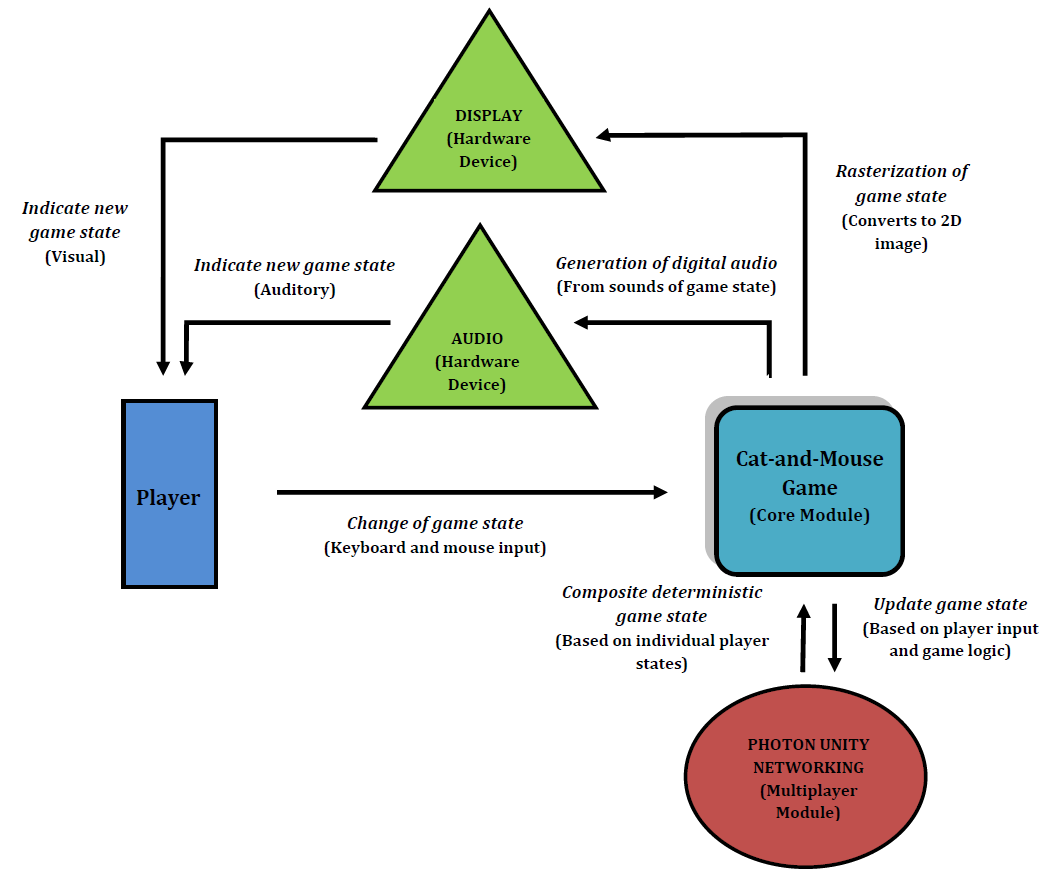
\includegraphics[width=\textwidth]{ContextDiagram.png}
\caption{Context Diagram for the Cat-and-Mouse Game}
\end{figure}
\newpage
\subsubsection{Work Partitioning}
\paragraph{}A list displaying all business events to which the game responds is indicated in \textbf{Table 2}. These 'real-world' events represent the general operations allowed in the game and indicates the action(s), if any, which should be taken.
\\
\\
\\ \textbf{Note:} The \textbf{"Input and Output"} for each \textbf{Business Event} in the Business Event List is:
\\
\\ \textbf{\emph{Change of game state (in); Update game state (out); Composite deterministic game state (in);  Rasterization of game state (out); Generation of digital audio (out); Indicate new game state - Visual (out); Indicate new game state - Auditory (out)}}
\\
\begin{longtable}{| p{0.40\textwidth}p{0.60\textwidth}|} 
\caption{\bf Business Event List for the Cat-and-Mouse Game}\\
\hline
{\textbf{Event Name}}  & {\textbf{Summary of BUC}}\\
\hline
\hline
\\
\printBusinessEvent  Player begins a new multiplayer session &  A new multiplayer session is started on the server.
\\
\hline
\printBusinessEvent  Player enters an existing multiplayer session & A new player is added to 'Lobby Screen' of the specified multiplayer session.
\\
\hline
\printBusinessEvent  Players select an open character slot on a Team & Each player is assigned to the their chosen character slot, if available. If the selected slot is already taken, it is indicated as such and the player must select another open slot.\\
\\
\hline
\printBusinessEvent  A single Player in a multiplayer session requests to start the match & Displays 'Player Ready' notification for that Player.\\
\\
\hline
\printBusinessEvent  All Players in a session request to start the match & The Players are assigned to their selected Teams and all players are placed ("spawned") within a randomly-generated Map Environment at the pre-defined Spawn Point for their respective Team.\\
\\
\hline
\printBusinessEvent  Player leaves the match & The  current match should continue if there are any remaining active players in the match. \\
\\
\hline
\printBusinessEvent  Player Character is moved & The Player's character is moved within the Map Environment.\\
\\
\hline
\printBusinessEvent  Player Character makes contact with the environment  & Depending on the type of environment, will affect the character's state in varying ways.\\
\\
\hline
\printBusinessEvent  Player Character requests the current location of the Character within the Map Environment. & The current position of a Player Character within the Map Environment, and in relation to other Player-Controlled and Environment-Controlled Characters, Map Objects, Objectives and Tasks should be indicated through a Map in the Heads-Up Display.\\
\\
\hline
\printBusinessEvent  Player Character is near an Item & The character is able to pick up the Item.\\
\\
\hline
\printBusinessEvent  Player Character is near an Item & The character is able to pick up the Item.\\
\\
\hline
\printBusinessEvent  Player Character is within the range of a Interactive Object. & The Character is able to utilise the Interaction Key to perform a (selection) of pre-defined behaviours on the object. \\
\\
\hline
\printBusinessEvent  Player Character picks up Item & The Item's effects (if any) are transferred to the Character. This may include changes in the Player's Vitality, Skills and Match Points of the Player's Team.\\
\\
\hline
\printBusinessEvent  Player Character makes contact with another Player Character from the same Team & Both players' movement is stopped.\\
\\
\hline
\printBusinessEvent  Player Character makes contact with Monster Character & Will drain the Health Points (HP) of the Player Character. May also inflict other effects on either of the Characters depending on each Character's respective Skills and Attributes.\\
\\
\hline
\printBusinessEvent Player Character makes contact with another Player from the opposing Team & Both Players' movement is stopped. Other effects may take place dependent on each character's respective Skills and Attributes.\\
\\
\hline
\printBusinessEvent  Player Character starts a Task within an active Match & Players provided with specific conditions which must be furfilled.\\
\\
\hline
\printBusinessEvent  Player Character finishes Task & Players granted enhanced Attribute(s), Skill(s), Items and/or Match Points.
\\
\hline
\printBusinessEvent  Player Character attacks another Player Character from the same Team & Nothing occurs.\\
\\
\hline
\printBusinessEvent  Player Character attacks another Player Character from the opposing Team & Will drain the Health Points (HP) of the opposing Player Character (dependent on Attributes and Skills). May also inflict other effects.\\
\\
\hline
\printBusinessEvent  Player Character attacks Monster  & Drains the Health Points (HP) of the Monster. May also inflict other effects.\\
\hline
\printBusinessEvent  Player Character beats Monster & Grants Player Character with enhanced Attribute(s), Skills(s), Items(s) and/or Match Points.
\\
\hline
\printBusinessEvent  Player Character uses Skill & Affects the attributes of the Player Character and/or the envrionment around them (including other characters). May trigger a Skill Cooldown Period (if applicable).\\
\\
\hline
\printBusinessEvent  Player Character gains enough Experience Points to advance a Level. & If the Character is not currently at the Maximum Permissible Level, the Player is advanced one Level, granted one additional Skill Point, and has their Health Points set to full and Experience Points set to empty.\\
\\
\hline
\printBusinessEvent  Player Character selects to learn a Skill & If the Character has the requsite number and type of Skill Points to acquire the desired Skill, and they have not previously obtained that Skill, the Skill is added to their Skill Bar and made available for use. Information regarding the behaviours and intended duration of the Skill should also be indicated to the Player. \\
\\
\hline
\printBusinessEvent  Player Character selects to view or modify their current Skills during an active Match.  & Skill information and modification dialogs should be displayed through the activation of a pre-defined of utility input sequence (Combination of Mouse and Keyboard input). \\
\\
\hline
\printBusinessEvent  Player Character selects to view the current status of and utilise their Attributes and Skills. & The game displays a Heads-Up Display (HUD), which displays basic Attribute and SKill information and allows for the use and/or activation of these attributes and skills.\\
\\
\hline
\printBusinessEvent  Player Quits the game  & Player is disconnected from the server and the game returns to the "Main Menu".\\
\\
\hline
\hline
\\
%No user input Business events
\printBusinessEvent  Monster attacks Player Character & Drains the Health Points (HP) of the Player Character. May also inflict other effects. \\
\\
\hline
\printBusinessEvent  Player Character's Health Points (HP) reaches zero & The Player Character will die.\\
\\
\hline
\printBusinessEvent  Player Character dies & The Player Character will be returned to the "Match Room Screen" of the Multiplayer Hub.\\
\\
\hline
\printBusinessEvent  All Player Characters on a Team are beaten.  &  The current match will end. The team with the most Match Points is declared to the the "Winner" of the current Match. All Players will be returned to the "Match Room Screen" for the session.\\
\\
\hline
\printBusinessEvent  Player disconnects from the server & The player will be returned to the "Main Menu". An error message is displayed.\\
\\
\hline
\printBusinessEvent  All Players have left the multiplayer session & The session (and all connections) will be closed.\\
\\
\hline
\hline
\\
% No multiplayer input Business events
\printBusinessEvent  Player starts the Cat-and-Mouse Game &  Displays the "Main Menu". Options to "Start Game", access "Options", and "Quit Game".\\
\\
\hline
\printBusinessEvent  Player selects the "Options" Menu from the Main Menu & Allows the Player to adjust various settings for the game (eg. graphics, audio, gameplay, etc).\\
\\
\hline
\printBusinessEvent  Player selects the "Quit Game" option from the Main Menu & Allows the Player to terminate the game.\\
\\
\hline
\hline
\end{longtable}
\newpage
\subsubsection{Individual Product Use Cases}
\paragraph{}Ideally, the user would receive the game from an online source such as a game distribution platform such as Steam, where they would download the game and install it. Individually, the game cannot be played but when they join the game's online rooms they will be able to find other players also looking for games to join. The user will then be able to play the game with other people online. 

\paragraph{}\textbf{Note:} \emph{The Cat-and-Mouse Game} refers tothe client-side and multiplayer aspects of the game. The server-side is provided thorugh the \emph{Photon Unity Networking} service. 
\subsection{Functional Requirements}

\textbf{Requirement 1:}  The Cat-and-Mouse Game should allow players to adjust in-game options (such as graphics, audio, the UI and gameplay settings) to suit their preferred experience and hardware.
\\
\textbf{Rationale:}  This will allow for the product to be accessible to a broader audience as well as a wider variety of hardware.
\\
\textbf{Fit criterion:}  Players have the ability to set the graphics fidelity in-game to match their computer's capabilities, toggle audio (background music, sound effects), as well as personalise the placement of various elements of the User Interface to their liking.
\\
\\
\\ \textbf{Requirement 2:}  The Cat-and-Mouse Game should allow players to join a Multiplayer Hub located on a server wherein they can create or join an existing Multiplayer Session ("Room").
\\
\textbf{Rationale:}  This will allow Players participate in the team-based aspect of the game, through joining multiplayer matches hosted on a remote server. 
\\
\textbf{Fit criterion:}  Players are able to connect successfully to the game server,  and create or join an existing match.
\\
\\
\\ \textbf{Requirement 3:}  The Cat-and-Mouse Game should allow players to select the Team they wish to join for the current Match.\\
\textbf{Rationale:}  This enables players to participate in Matches with selected users (or new users). This encourages closer team cohesion and collaboration with individuals whom a player may work well with, as well as provide an oppotunity to play with new players.
\\
\textbf{Fit criterion:}  Players are able to select a Character Slot on the Team which they prefer to play on for the current Match, and will be placed into that slot if it is available.
\\
\\
\\ \textbf{Requirement 4:}  The Cat-and-Mouse Game should allow players to request to start the current Match.\\
\textbf{Rationale:}  This enables players to enter the "Ready" State and indicate to other players that they have made their Team Selection and is ready to enter the map environment. \\
\textbf{Fit criterion:}  A "Player Ready" notification is displayed in addition to the Player Name next to their selected Character Slot on a Team.
\\
\\
\\ \textbf{Requirement 5:}  The Cat-and-Mouse Game should allow all players to enter the Map Environment when all Players within the current Match have requested to start the Match.\\
\textbf{Rationale:}  This allows for players to enter the Map Environment and interact with each other upon all Players indicating their readiness to start the Match. \\
\textbf{Fit criterion:} The Players are assigned to their selected Teams and all players are placed ("spawned") within a randomly-generated Map Environment at the pre-defined Spawn Point for their respective Team.
\\
\\
\\ \textbf{Requirement 6:}  The Cat-and-Mouse Game should provide multiple objectives, character attributes, character skills and game-modes within each Match.\\
\textbf{Rationale:}  To appeal to a wide audience, players should have the freedom to adapt their gameplay experience according to their interests, skill level and play style.\\
\textbf{Fit criterion:}  Players are able to participate from a variety of abilities, skills, objectives, maps and game modes to fit their personal prefrences. The two different Teams should also have varying attribute and Skill behaviours and progression paths. 
\\
\\
\\ \textbf{Requirement 7:}  The Cat-and-Mouse Game should allow players to see and interact with each other through avatars in real-time to complete tasks and obectives within a virtual maze. \\
\textbf{Rationale:}  This aspect enables key collaborative elements around which the core mechanics and gameplay have been designed.\\
\textbf{Fit criterion:}  Individuals are able to see the position and status of, as well as interact with the virtual environment simultaneously with the other players participating in the match.
\\
\\
\\ \textbf{Requirement 8:}  The Cat-and-Mouse Game should allow players to move their characters around the map as the environment allows. \\
\textbf{Rationale:}  Ensuring freedom of movement encourages players to be adventurous and creative in their interactions with not only the game objectives, but other fellow participants as well.\\
\textbf{Fit criterion:}  Individuals are able to move to any point in the map (subject to the laws of physics as defined by the Physics module and defined boundaries).\\
\\
\\
\textbf{Requirement 9:}  The Cat-and-Mouse Game should allow players to attack and deal damage to the corresponding players on the opposing team though regular attacks and Skill-based attacks and effects. \\
\textbf{Rationale:}  This allows for game progression, and encourages team cooperation by introducing a survival element to the gameplay.\\
\textbf{Fit criterion:}  Players are able to wield various attack and defensive skills to cause damage and/or negative effects to a player on the opposing team. The ability to utilise  skills may be regulated by a Skill Cooldown indicator, which indicates the remaining time until the next possible use of the Skill . Remaining Health is also indicated and upon reaching a Health Point value of 0, the player "dies" and is (temporarily) unable to participate further in the match. The victorious Player will be granted increased Vitality attributes in addition to Match Points.
\\
\\
\textbf{Requirement 10:}  The Cat-and-Mouse Game should allow players to attack and deal damage to the Monsters within the Map though regular attacks and Skill-based attacks and effects. \\
\textbf{Rationale:}  This allows for game progression, and encourages team cooperation by increasing the survival element within the game.\\
\textbf{Fit criterion:}  Players are able to wield various attack and defensive skills to cause damage and/or negative effects to a Monster within the Map Environment. The ability to utilise  skills may be regulated by a Skill Cooldown indicator, which indicates the remaining time until the next possible use of the Skill . Remaining Health is also indicated and upon reaching a Health Point value of 0, the monster will die, and (may) be respawned after a certain period of time. The victorious Player will be granted increased Vitality attributes in addition to Match Points.
\\
\\
\\ \textbf{Requirement 11:}  The Cat-and-Mouse Game should allow teams to gain points through acomplishing certain in-game tasks or objectives.\\
\textbf{Rationale:}  This allows for game progression, and a the competitive element encourages greater team cohesion in order to get ahead. Furthermore, a variety of objectives and paths towards progression encourages greater creativity with regards to developing unique play-styles and fosters team collaboration to advance the Team thorugh the completion of many different tasks simulataneously. The latter also facilitates deeper and longer-term player engagement thorugh a diversity in available activities.\\
\textbf{Fit criterion:}  Each team is granted points for accomplishing certain objectives over the course of a match. Dependent on the mode and parameters of the match, the game is considered "won" either when a Team attains the highest number of points after a certain period of time, a special condition has been fulfilled (e.g. capture the flag), or all members of the opposing Team have been eliminated.  
\\
\\
\\ \textbf{Requirement 12:}  The Cat-and-Mouse Game should allow teams to gain points through collecting various objects placed thorughout the Map Environment.\\
\textbf{Rationale:}  This allows for game progression, and a the competitive element encourages greater team cohesion in order to get ahead. Furthermore, a variety of objectives and paths towards progression encourages greater creativity with regards to developing unique play-styles and fosters team collaboration to advance the Team thorugh the completion of many different tasks simulataneously. The latter also facilitates deeper and longer-term player engagement thorugh a diversity in available activities.\\
\textbf{Fit criterion:}  Special objects are placed randomly throughout the Map Environment that when picked up, grants a number of Match Points to the Player's Team. The object may (or may not) be continue to be collectable after being picked up by a Character. 
\\
\\
\\ \textbf{Requirement 13:}  The Cat-and-Mouse Game should allow teams to interact with Interactive Objects placed within the Map Environment.\\
\textbf{Rationale:} This allows for an additional dimension of interaction within the Map Environment when completing match objectives. This increases the level of fidelity and player engagement within the Match. \\
\textbf{Fit criterion:}  Special objects are placed randomly throughout the Map Environment that when the Player is within the range of, allows for the execution of (several) pre-defined behaviours on the object which modifies the Map Environment in some manner. 
\\
\\
\\ \textbf{Requirement 14:}  The Cat-and-Mouse Game should ensure that all players start on an even level playing field, so that there is a lower barrier of entry for new and casual players.\\
\textbf{Rationale:}  The social nature of the game and strong focus of the game around teamwork and cooperation is such that the need for such skills to succeed should not be mitigated by the sheer amount of time spent in-game.\\
\textbf{Fit criterion:}  Limited or no game state data is retained upon the termination of a multiplayer session. When starting a new game, previous player performance and accomplishments do not impact the skills or abilities which are granted to a player. Although both the 'Cat' and 'Mouse' Teams host varying Skills and Attributes, the game mechanic will be balanced so that neither team has a predetermined advantage over the other.
\\
\\
\\\textbf{Requirement 15:}  The Cat-and-Mouse Game should allow for opportunities for Players to enhance their Skills and Attributes through various in game interactions, such as by completing quests, defeating Monsters and collecting Items and Consumerables.   \\
\textbf{Rationale:}  The ability (and indeed, necessity) for a Player to work their way up from baseline in every session motivates individuals to fully explore all the possbilities which are present in every situation. Thus, all participants will be fully engaged in the game experience, and newcomers to the game will not be at a disadvantage in term of enjoyment (e.g. in terms of more 'experienced' players using the same skills over and over again in every match).\\
\textbf{Fit criterion:}  All Players are able and encouraged to interact with the game envrionment (and other players) in new and innovative ways in every match, and a variety of different paths to the same goal will provide for high replay value for even the most seasoned players. This interaction should lead to the advancement of the Player's Attributes and/or Skills.
\\
\\
\\ \textbf{Requirement 16:}  The Cat-and-Mouse Game should allow for opportunities for Players quit the Current Match without terminating the Match for any Players still active within the Room.\\
\textbf{Rationale:}  This allows for players to leave an active match without other team members and players incurring negative effects (excluding the potiential loss of a team member). This decreases the chance of negative perceptions towards players developing within the community.\\
\textbf{Fit criterion:}  Upon the choice to quit the Current Match being made, a disconnection from the Match Room or any other operational events occurring which causes a Player to be disconnected from the Match Room, the other Players continue to remain in the Match Room (or Map Environment if the match is active), with no change in their status or the game state.
\\
\\
\\\textbf{Requirement 17:}  The Cat-and-Mouse Game should terminate a match upon the fulfillment of one or more pre-defined condition(s).\\
\textbf{Rationale:}  This enables match progression to lead to one or more "end-game goals". This increases player engagement and thus, encourages greater team and player co-operation towards a shared goal. \\
\textbf{Fit criterion:}  The following conditions will result in the ending of the Match. The team  with the most Match Points is then declared to be the Winner. All Players are then returned to the Match Room Screen for the current multiplayer session: (i)  \emph{Upon the defeat (or exit from the Match) of all members of the opposing Team}; (ii) \emph{Upon the exit from the Maze component of the Map Environment by all members any team, as indicated by designated exit points.}  
\\
\\
\\\textbf{Requirement 18:}  The Cat-and-Mouse Game should not allow for members of the same Team to deal damage to one another.\\
\textbf{Rationale:}  This facilitates greater cohesion, co-coperation and commanderie between members of a Team, and decreases the chances of tension and/or disagreement.   \\
\textbf{Fit criterion:}  When a member of a Team utilises an attack or skill directed towards or within the vicinity of another Player of the same Team, any effects which decrease the Health Points of the latter Character is negated.
\\
\\
\\ \textbf{Requirement 19:}  The Cat-and-Mouse Game should enable the effects of Skills which carry benefits to nearby Characters or members of the same Team to affect the attributes and Skills of these Players.\\
\textbf{Rationale:}  This promotes positive team collaboration and mutual assistance between players. Individuals are also more likely to adopt an approach which provides the best advantage to the entire team, and correspondingly less likely to engage in behaviours which only provide \emph{self-satisifying} benefits.  \\
\textbf{Fit criterion:}  When a member of a Team utilises a supportive Skill with an \emph{area of effect} or \emph{which is directed towards one or more team members} some or all of the effects of that Skill is applied to the applicable Characters.
\\
\\
\\ \textbf{Requirement 20:}  The Cat-and-Mouse Game should define certain areas of the Map Environment which apply one or more effects to nearby Players on passage of some area and/or trigger of some condition by a Character. \\
\textbf{Rationale:}  This increases the dynamicity and interactivity of the Map Environment, which in addition to increasing the intensity and duration player engagement, further fosters team coordination to devise unique solutions to the obsticles posed by these effect(s) .  \\
\textbf{Fit criterion:}  When a Character enters a designated area or block within the Map Environment, one or more effects will be applied to their attributes and/or Skills, such as decreasing their flexibility of motion or Vitality.
\\
\\
\\ \textbf{Requirement 21:}  The Cat-and-Mouse Game should provide for common gains and losses with regards to certain attributes within a Team.  \\
\textbf{Rationale:}  This increases the actual and perceived benefit of greater team co-operation and cohesion, while introducing penalties for a solo and self-satisfying approach. This will also encourage each individual to contribute to the overall performance of the Team by utilising their individual areas of strength to complete tasks and objectives.  \\
\textbf{Fit criterion:}  Experience points within a Character's Vitality attributes are shared between all members of the Team. Thus, character Level Progression and acquisition of additional Skills and attributes are closely correlated to the performance of the Team as a whole, rather than any one specific individual.
\\
\\
\\ \textbf{Requirement 22:}  The Cat-and-Mouse Game should provide a secondary, non-instrusive interface to view and modify Character Attributes and Skills.  \\
\textbf{Rationale:} Due to the fast-paced, survival-centric nature of the game, as well as the input methods and layout available to the Player, a seperate (series) of interfaces should be provided, disjoint from the main Heads Up Display (HUD), the latter which indicates the status of and allows for the use the Character's basic Attributes and Skills.  \\
\textbf{Fit criterion:}  A (series) of dialog boxes, seperated and visually distinguishable from the HUD, allows for the Player to view detailed descriptions relating to the status and behaviour of their Character's attributes and learned Skills. Additionally, through these dialog boxes, users are able to make additons and modifications with regards to these attributes and Skills, dependent on the completion of certain match objectives. The activation of these secondary interfaces is through a combination of Mouse and Keyboard commands, in a \emph{moded} configuration.
\\
\\
\\ \textbf{Requirement 23:}  The Cat-and-Mouse Game should provide a Heads-Up Display, visible on the primary interface upon the start of a Match, which indicates the status of basic Character Attributes and Skills, as well as enables for their activation and/or use as desired by the Player. \\
\textbf{Rationale:} Due to the fast-paced, survival-centric nature of the game, rapid access to basic information regarding the status of a Character's primary attributes and skills, as well the latter's as streamlined distinguishability and activation by the Player is crucial to the effectiveness of the game in conveying its intended message(s). This is as the former  enables for the rapid acqusition of the most important operational concepts and requisite knowledge required by the Player to facilitate  full and effective participation in the game. Correspondingly, this leads to a maximisation of a Player's attention and resources on team collaboration and coordination to complete the core game tasks and objectives, while limiting any potiential frustration and time spent on the logistics of the interface. \\
\textbf{Fit criterion:} A few prominent and easily-distinguishable Interface Bars, Labels and other indicators display to the user the current status of the Character's primary Attributes (such as Level, Health and Experience Points). In addition, a Skill Bar allows for the user to view currently learned and available Skills, as well as enables for their rapid use through the activation of pre-defined hotkeys designated to each Skill Slot.
\\
\\
\\ \textbf{Requirement 24:}  The Cat-and-Mouse Game should provide a Minimap which indicates the current position of the Player, in relation to other Player-Controlled and Environment-Controlled Characters, major geographical features, interactive objects and task or objective-related locations, characters and/or items. \\
\textbf{Rationale:} Due to the fast-paced, survival-centric nature of the game, rapid access to basic information regarding the status of a Character's location in relation other Characters, as well as major features, within the Map Environment provides direction to Players regarding the location of their team members, enemy players and monsters. as well as  regarding the tasks and objectives of the Match. This facilitates team coordination and strategic planning, in addition to minimsing any potiential sources of player confusion and frustration. \\
\textbf{Fit criterion:} A few prominent and easily-distinguishable Interface Bars, Labels and other indicators display to the user the current status of the Character's primary Attributes (such as Level, Health and Experience Points). In addition, a Skill Bar allows for the user to view currently learned and available Skills, as well as enables for their rapid use through the activation of pre-defined hotkeys designated to each Skill Slot.
\\
\\
\\ \textbf{Requirement 25:}  The Cat-and-Mouse Game should provide easily visible and distinguishable messages to the Player indicating the conditions of various Match Tasks and Objectives, as well as the status of any Tasks and Objectives which are currently in-progress or active. \\
\textbf{Rationale:} Due to the fast-paced, survival-centric nature of the game, strealined access to information regarding the availiblity and status of Tasks and Objectives within the Map Environment sets the framework for effective teamwork and mutual formation and understanding of the goals of the Team. This further encourages positive social interactions and co-operation between Team Members, while limiting any potiential for frustration. Additionally, the provision of relevant information aiding match progression provides context for the data provided to the Player by the Heads-Up Display and the Minimap, as well as assists in future planning and decision-making processes regarding the selection of Skills and paths for character progression.  \\
\textbf{Fit criterion:} Clearly-contrasted text in large-font and bright colours is displayed on the primary interface upon the start of a Match and  the commencement of major tasks, objectives, events and/or  the triggering of certain conditions, so as to provide guidance and critical information to Players relating to the successful navigation of these elements within the Map Environment. The finer details will be omitted from these messages, in order to encourage critical and creative thinking, as well as team cooperation. A Game Manual will also be provided to provide a basic control, mechanics and objective reference to players. 
\\
\\
\\

\section{Non-Functional Requirements}
\subsection{Look and Feel Requirements}
\subsubsection{Appearance Requirements}
\paragraph{}The game's interface shall be attractive to audiences of all ages and customers should be able to easily and quickly use the interface as it will be as intuitive as possible. We will use darker colours for the most part, avoiding flashy or warm colours in favour of colder colours to match the labyrinth theme and to help create a sense of tension.  
\subsubsection{Style Requirements}
\paragraph{}We want this game to appear simple and intuitive, so that it does not intimidate certain age groups. However, it will have a mature look to it and a western art style, and together they will create a intense, dungeon-like feel. The players should feel a light sense of tension when playing, the Cat because he wants to find the Mice as soon as possible and the Mice because they do not want to be found.  
\subsection{Usability and Humanity Requirements}
\subsubsection{Ease of Use Requirements}
\paragraph{}The product will be easy to use for users of all ages, requiring basic English skills and use of a computer mouse and keyboard. The user should be able to learn the basic concepts and components of the game very easily, namely the controls, core mechanics, and the objective of the game, through simple on-screen messages, as well as by refrencing the included Game Manual. 
\subsubsection{Personalization and Internalionalization Requirements}
\paragraph{}The basic controls will be customizable, allowing the user to change certain hotkeys to whatever they please. The interface will be semi-customizable, allowing the user to move or resize items to their preference. 
\paragraph{}The first release of the product will only support English, but it will be written in simplistic and easy-to-understand diction such that even individuals not fluent in English will be able to quickly grasp the basics of the game. Upon further development, we may include language packs such as Chinese and French. 
\subsubsection{Learning Requirements}
\paragraph{}Even though the game will be designed to be easy to learn, and easy to get a basic feel of the game, it will be very hard to master. Playing this game at the highest level will require the user to memorize the most efficient paths or abilties, and make very few errors in terms of gameplay. The game should be difficult enough to inspire motivation to improve, but also easy enough to avoid discouraging users from playing. A benchmark will be such that a new user will have a general feel of the game after going through the tutorial, but becoming a master at the game will take hundreds of hours of gameplay. The game should have a lasting impression on the users in terms of fun and desire to improve, and make them want to come back and play again. 
\subsubsection{Understandability and Politeness Requirements}
\paragraph{}Since the product is a video game, there will be concepts that are foreign to non video game players. However, the basic concept of the game is designed around the game "cat and mouse" which most people should be familiar with; a game where the cats try to catch the mice. A tutorial will be included in the game, and will be written in a way that is easy to understand for anyone, avoiding difficult concepts or jargon when possible, and explaining them in detail when required. 
\subsubsection{Accessibility Requirements}
\paragraph{}As a video game, the physical aspect cannot be easily substituted as the user will always be required to control their character using a keyboard and mouse, or a modified controller. The visual aspect also cannot be replaced as the user is required to be able to see everything that is going on in game, so fully blind individuals will unfortunately be unable to use this product. However, we can provide options for the colorblind by changing the in game colors to suit their needs. To suit the needs of the deaf, we can have subtitles of annotations for them to read. 
\subsection{Performance Requirements}
\paragraph{}We hope to target players of all demographics, and we hope that they will be able to enjoy our game even if they do not have the latest computer systems. We will thus design our game to run smoothly on older computers as well as newer models.
\subsubsection{Speed and Latency Requirements}
\paragraph{}As the game operates at a real time level and is also multiplayer, we want each player to constantly have updates on the current game state. This would require information packets to be sent to each player multiple times every second, and each group of packets will contain information such as other the movements or actions of other players. The users will therefore be required to have a minimum internet connection speed of 1 Mbps. This latter bandwidth requirement will ensure for a stable connection and effective communication between the user's computer and the Multiplayer Servers.
\paragraph{}Latency is also an important issue to consider in a real-time game such as the one we are developing. Players need to be able to react immediately to what is going on in the game, so their latency should be as low as possible. We will aim to limit the ping between each player to the Multiplayer Server to be 100 ms or less, as any more than this causes an obvious delay between the user's physical actions and their characters actions. This latter latency limit assumes an average frame-rate of 30 Frames Per Second, as well as a \emph{sync packet} requested once every frame, thus enabling  successful synchronisation between the client and server at least once every 5 frames, accounting for a 40 \% margin of error on synchronisation requests.
\subsubsection{Safety-Critical Requirements}
\paragraph{}The game will not have any extremely flashy effects that can cause seizures for certain individuals. 
\subsubsection{Precision or Accuracy Requirements}
\paragraph{}N/A.
\subsubsection{Reliability and Availability Requirements}
\paragraph{}The server that a user hosts should not fail until said user closes it themselves. If the user leaves the game but does not close the server, then it should persist. The game itself should also not crash under any circumstance.
\subsubsection{Robustness or Fault-Tolerance Requirements}
\paragraph{}If a server is shut down unexpectedly, the game should kick players and display an error message to let them known what has happened. Any other unexpected errors should also display a message to the clients. If any player leaves the game, the game should continue as usual and switch a player to the other team if it is unbalanced.  
\subsubsection{Capacity Requirements}
\paragraph{}Each game instance will host up to four players at a time, and information for each player will need to be stored on the server at any given time. For each user, the game will need to receive and hold data on each of the other three players as well as the current game state. 
\subsubsection{Scalability or Extensibility Requirements}
\paragraph{}If the game increases in popularity then our servers will need to be upgraded to handle the increased traffic. The game itself will also be able to handle frequent patches to fix bugs or add new features. 
\subsubsection{Longevity Requirements}
\paragraph{}As a computer video game, the expected lifetime of the product is as long as the user is interested in playing. A typical user can be expected to play for 1-2 hours, however if frequent updates are made to the game and the user constantly finds it fun, then the game's lifetime can be much longer. 
\subsection{Operational and Environmental Requirements}
\subsubsection{Expected Physical Environment}
\paragraph{}N/A.
\subsubsection{Requirements for Interfacing with Adjacent Systems}
\paragraph{}This game should work with Windows 7, 8, 8.1 and 10. It should also work with DirectX 11 and DirectX 9 as those are the graphics API that we will be using with Unity. 
\subsubsection{Productization Requirements}
\paragraph{}This product will require users to have either DirectX 9 or DirectX 11 installed. The product will be distributed as a ZIP file, all users need to do is unzip it.
\subsubsection{Release Requirements}
\paragraph{}Ideally the game will be released on a game platform such as Steam, which allows users to receive updates with ease. However the first versions of the game will be released as a downloadable bundle where the user will have to download and install manually, then open the game by running the executable files. 
\subsection{Maintainability and Support Requirements}
\subsubsection{Maintenance Requirements}
\paragraph{}Patches and updates will be released as the creators see fit, in order to address bugs in the game, issues with balancing, or to release new game content. 
\subsubsection{Supportability Requirements}
\paragraph{}The game will require minimal support, however if the user encounters issues with the game then they can contact the creators directly to look for a fix. 
\subsubsection{Adaptability Requirements}
\paragraph{}Currently, we do not plan on porting the product no other platforms or environments.
\subsection{Security Requirements}
\subsubsection{Access Requirements}
\paragraph{}The users will only be able to access the main game and the options that we see fit. The source code and server code will be hidden and restricted from the user. 
\subsubsection{Integrity Requirements}
\paragraph{}Serious damage can be caused if an outsider gains access to the source code, so steps will be taken to prevent unauthorized access. Hacking into the servers can also cause issues with cheating and players gaining unfair advantages, so steps will also be taken to stop outside attacks. 
\subsubsection{Privacy Requirements}
\paragraph{}This game will not have private information stored. The only information a user will have is their username, which will be stored on the client's machine.
\subsubsection{Audit Requirements}
\paragraph{}N/A.
\subsubsection{Immunity Requirements}
\paragraph{}Users having anti-virus software should be sufficient for protection against unauthorized programs like viruses.
\subsection{Cultural Requirements}
\paragraph{}The product will not have anything offensive or sensitive, culturally or religiously. The game's primary language will be in English and is not intended for a market outside of the US and Canada.
\subsection{Legal Requirements}
\subsubsection{Compliance Requirements}
\paragraph{}All of our assets and code will be created by ourselves or royalty free.
\subsubsection{Standards Requirements}
\paragraph{}N/A.
\subsection{Health and Safety Requirements}
This section is not in the original Volere template.
\paragraph{}We do not want our game to use flashing imagery and effects that can potentially cause health issues such as seizures. This includes effects such as the game frequently flashing bright colors at the user, and use of certain patterns which can trigger an seizure in the affected demographics.
\section{Project Issues}
\subsection{Open Issues}
\begin{itemize}
    \item Finding a good balance to the game is an issue. Because teams are asymmetrical (there is only 1 cat, while there is 3 mice), and each team has different abilities, it's hard to gauge how fair it is for one team which can affect how much fun the players have playing this game. 
    \item Still need to think of an algorithm for map generation that makes the maps enjoyable to play on. 
\end{itemize}
\subsection{Off-the-Shelf Solutions}
\subsubsection{Ready-Made Products}
\paragraph{}N/A
\subsubsection{Reusable Components}
\paragraph{}N/A
\subsubsection{Products That Can Be Copied}
\paragraph{}There are asymmetrical player versus player games currently on the market, which if we could legally copy them, it could help with our game's potential balancing issue. A game that comes to mind is Evolve, which has one team being composed of a single player playing as a monster, and four hunters as the other team. Similar to ours, the teams have their own unique abilities and skillset. 
\subsection{New Problems}
\subsubsection{Effects on the Current Environment}
\paragraph{}N/A
\subsubsection{Effects on the Installed Systems}
\paragraph{}N/A
\subsubsection{Potential User Problems}
\paragraph{}N/A
\subsubsection{Limitations in the Anticipated Implementation Environment That May Inhibit the New Product}
\paragraph{}The game might not run optimally depending on the hardware a user uses to run it. 
\subsubsection{Follow-Up Problems}
\paragraph{}N/A
\subsection{Tasks}
\subsubsection{Project Planning}
\begin{itemize}
    \item Produce sufficient and necessary documents such as requirement document, user guide, etc. 
    \item Acquire necessary knowledge about tools we are using, and to familiarize ourselves with them. 
    \item Develop a playable prototype of the game without all the features yet. 
    \item Add on to the the prototype.
\end{itemize}
\subsubsection{Planning of the Development Phases}
\begin{itemize}
    \item Basic movement/controls of the characters.
    \item Map generation algorithm.
    \item Networking so multiplayer works.
    \item Creating the game's interfaces such as menus.
    \item Adding abilities and objectives to the game.
    \item Re-balancing the game after acquiring appropriate feedback from testers.
    \item Adding graphics and sounds that are not placeholders to polish the game's aesthetics.
\end{itemize}
\subsection{Migration to the New Product}
\subsubsection{Requirements for Migration to the New Product}
\paragraph{}N/A
\subsubsection{Data That Has to Be Modified of Translated for the New System}
\paragraph{}N/A
\subsection{Risks}
\begin{itemize}
    \item Certain abilities might be badly balanced, and thus make it unfair for one team.
    \item Procedurally generated maps using algorithms might affect balance of the game. 
    \item Might not be able to find enough play testers to give satisfying feedback.
    \item Could run into trouble with networking and making it playable online.
    \item Time could be badly managed, and will need to cut down on features.
\end{itemize}
\subsection{Costs}
\paragraph{}There will be a time cost of 7 months for development of the game, but will cost no money as all tools used are free.
\subsection{User Documentation and Training}
\subsubsection{User Documentation Requirements}
\paragraph{}We will provide a User Documentation, as it is required as part of our capstone. There will also be a tutorial in game that informs players about the rules and how to play the game. This tutorial will cover topics such as joining a game, joining a team, movements, and objectives of the game. 
\subsubsection{Training Requirements}
\paragraph{}The game will require users to know basic English in order to go through the tutorial and play the game.
\subsection{Waiting Room}
\paragraph{}A requirement that might be done after the initial release of the product is an installation wizard. For now we think it is best to stick with an executable file for the game. Using an installation wizard also gives us the option to use more external dependencies, and thus more features if needed. any further requirements that might be added will be listed here as the document is revised.
\subsection{Ideas for Solutions}
\paragraph{}Currently, we do not have any ideas for solutions. This might change as we update this document.
\bibliographystyle{plainnat}
\bibliography{SRS}
\end{document}